\chapter{Concept and Design}
\label{cha:conceptanddesign}

\section{General}

\section{Challanges}
\label{sec:challanges}

\subsection{Security Goals}
\label{sec:securityGoals}

Designing a identity management systems comes with various legal implications. We are referring here to § 9 “Technical and organizational actions” in the “Federal Data Protection Act”\footnote{Translated from the German language “Bundesdatenschutzgesetz”} were an identity management system shell enforce all necessary measures to protect identity information.\cite{bdsg}

So we will focus on the following security goals:
\begin{enumerate}
\item \textbf{Confidentiality:} Data shell be secured on its transmission. This includes the blockchain and communication over the internet. 
\item \textbf{Integrity:} The integrity of the data needs to be assured so that no entity can change identity information without knowledge. 
\item \textbf{Authenticity:} Identity information are protected against unauthorized access. 
\item \textbf{Non-Repudiation:} No entity can deny having taken an action.
\item \textbf{Privacy:} The privacy of a user is preserved while interacting with the system. 
\end{enumerate}

We further also see the blockchain as a world open readable ledger were everyone can read transactions or information stored on the blockchain. So interactions with the blockchain need to ensure to not expose any identity information. 
It is not allowed to store hashes or encryption of claim in the blockchain, since it is a tamper-proof data storage, information can not be removed once written. So if the hash or encryption gets broken the identity information is leaked and can not be removed.  

\section{Processes}

\subsection{Registration}

 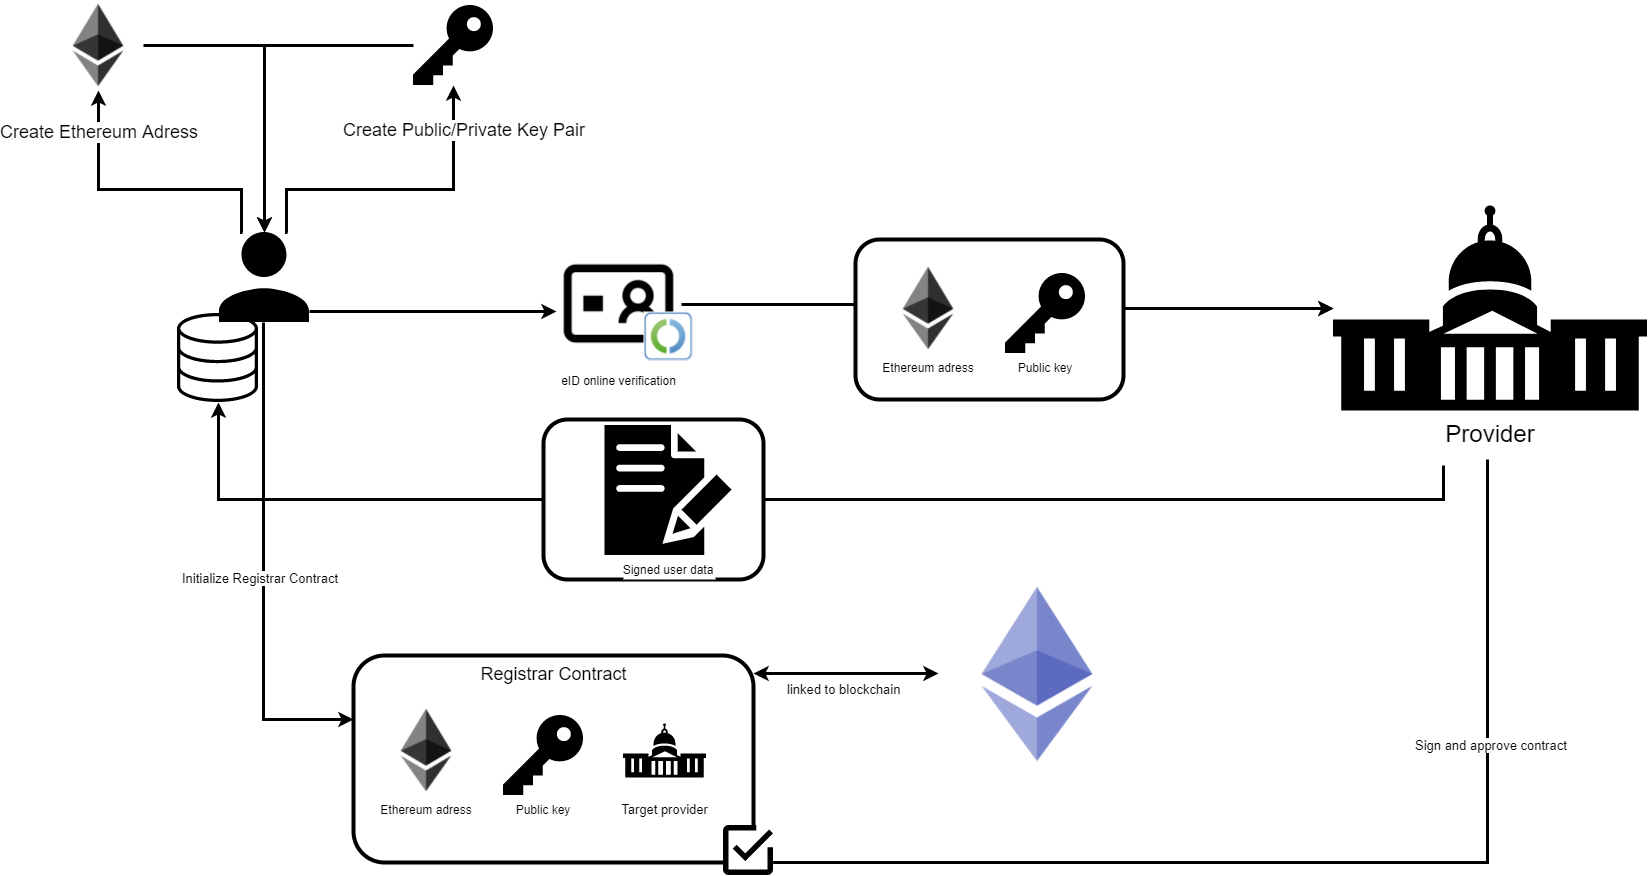
\includegraphics[width=\textwidth]{concept/registration.png}

\subsection{Permission Request}

 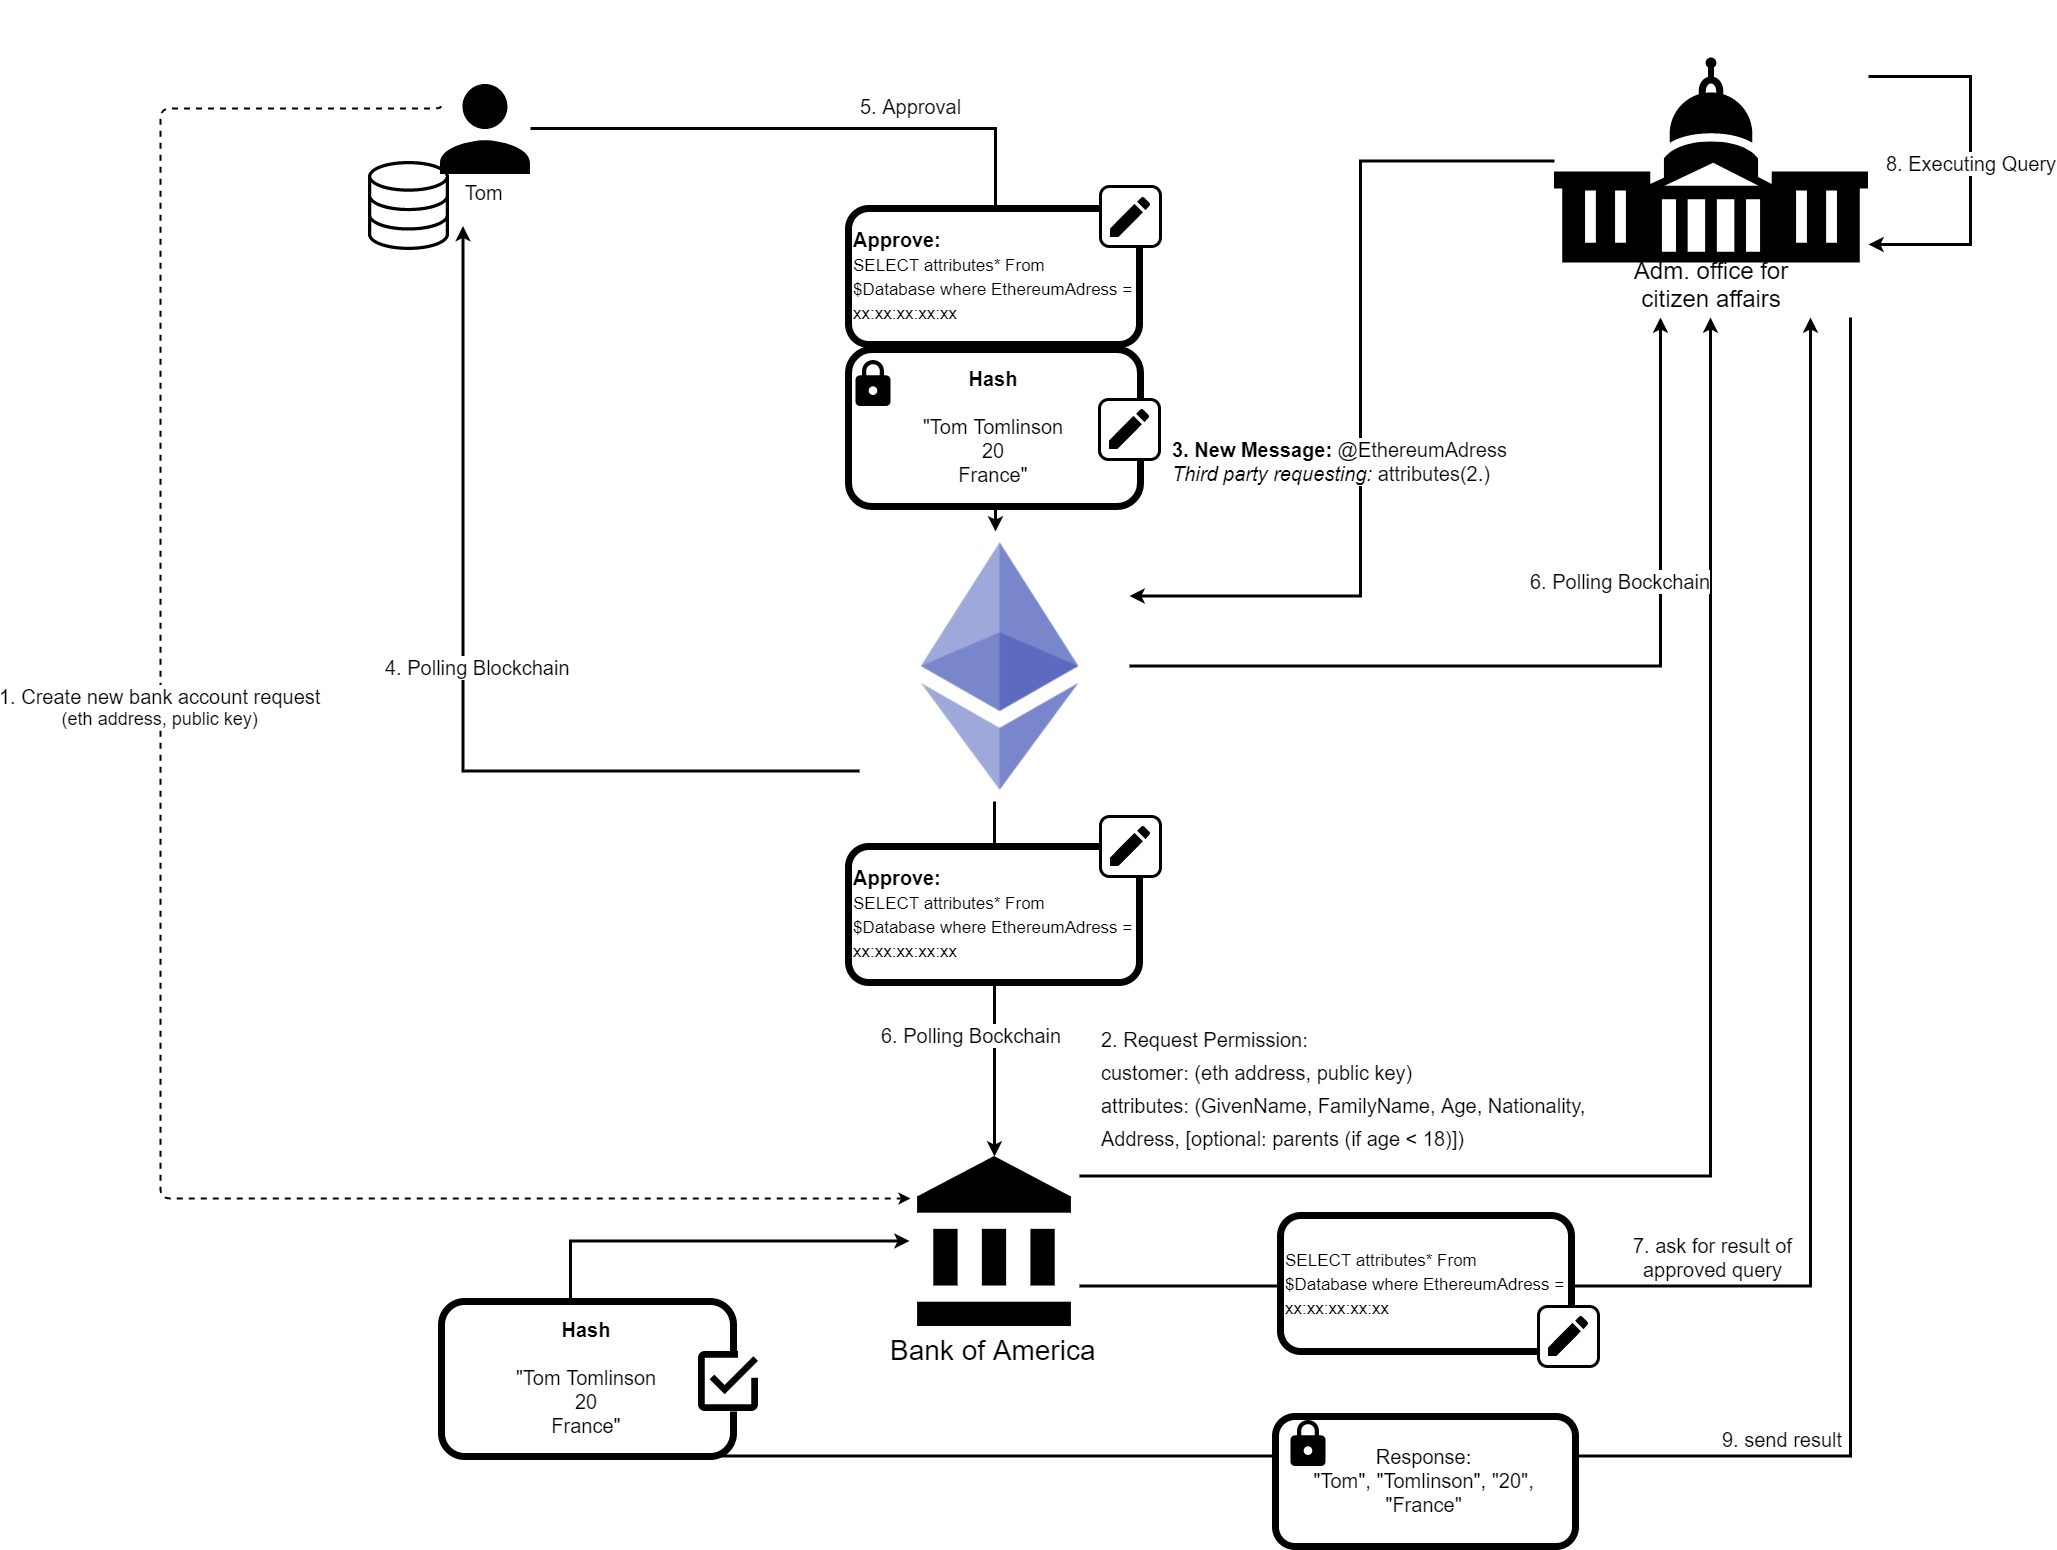
\includegraphics[width=\textwidth]{concept/permission_request_bank.png}

\subsection{Changing Attributes}

 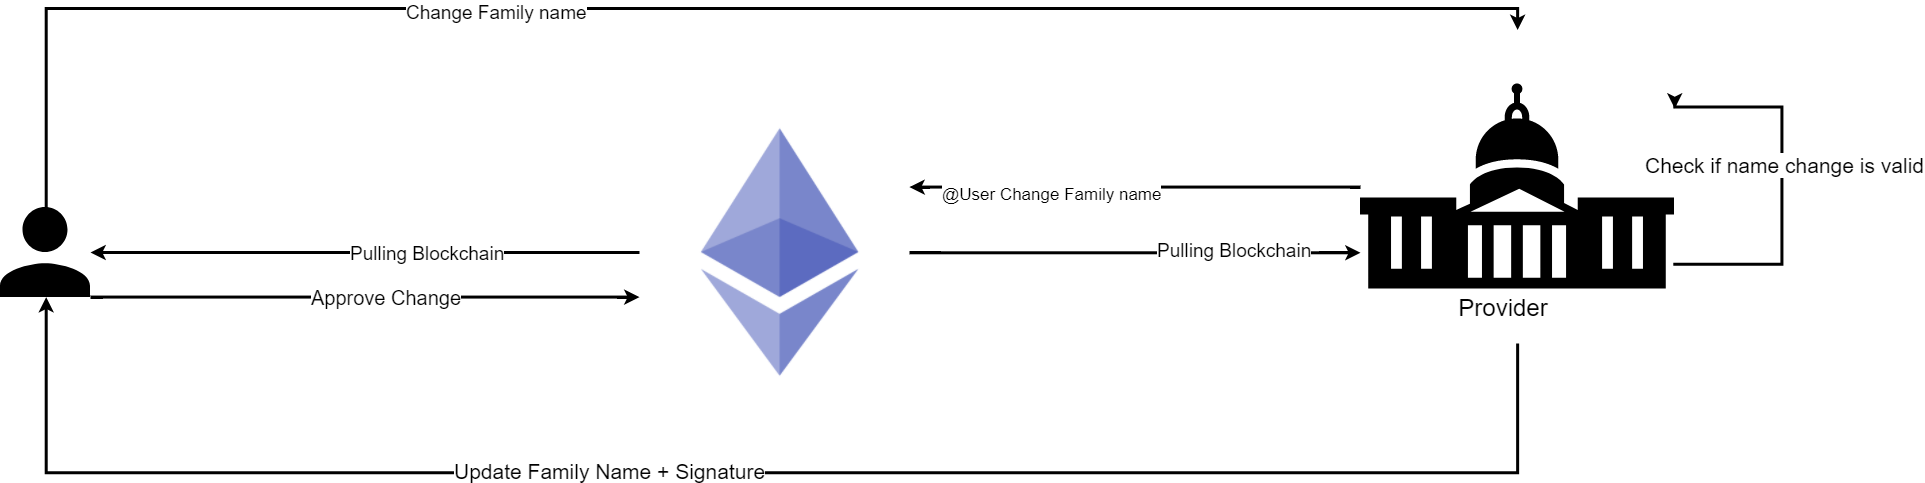
\includegraphics[width=\textwidth]{concept/change_attribute.png}

\subsection{Evaluation}

 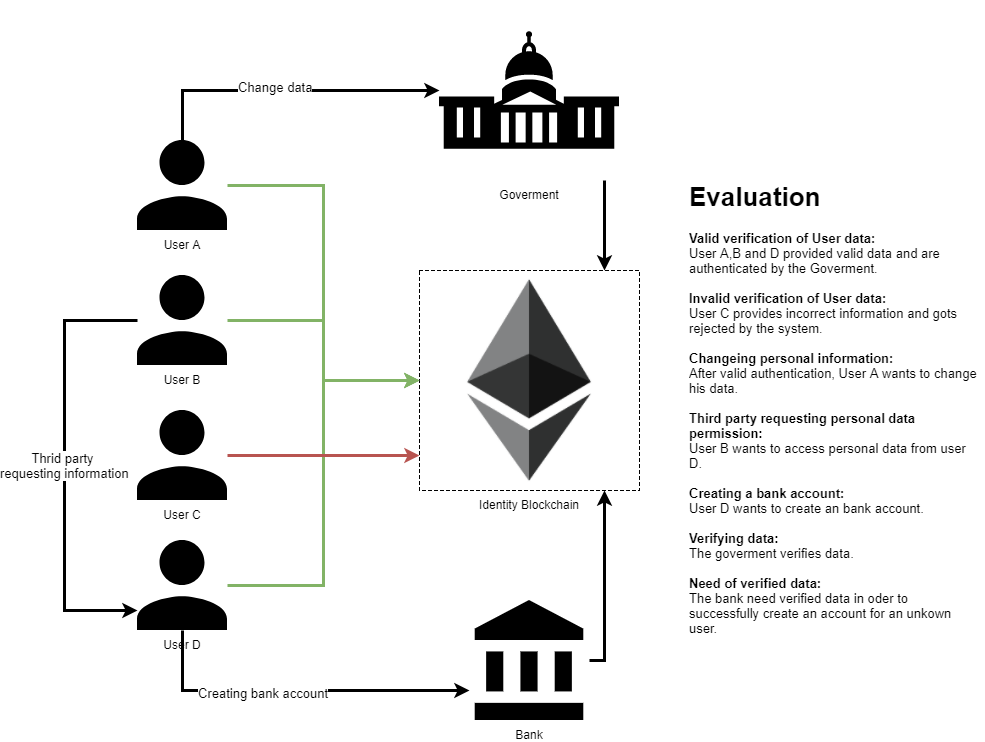
\includegraphics[width=\textwidth]{concept/evaluation.png}
 
\section{Use cases}

\subsection{Change a claim}
Lets have a user Bob Bobsen who has recently married Alice Alicson. Since Bob wants to change his family name to Bob Alicon this information needs to be updated in our system. To do so he sends a Update-Familiy-Name-Request with his new family name, to the corresponding identity provider, most likely the government. They on the other hand, can now verify this new claim by checking Bob's marriage contract. If all information match Bobs claims the identity provider publishes a Change-Family-Name-Claim transaction in the transaction blockchain to notify all third parties and other identity providers about the new claim of Bob's ID. 
Bob does then pull the blockchain, verifies the transaction code and approves the change by publishing his approval to the blockchain. The government permanently changes Bobs name in their database and sends the changes to Bob so that he can store the same changes in his local database. 
Each provider also holding bobs family name can then query the identity provider issued the name change again to pull the new name of Bob if Bob permitted this. (He could have done so by setting the "reuse" flag in the header of his signed query.)
The process described above will be processed in the same way when a third party requests a change of a claim. Bob on the other hand needs to explicitly approve this change. To model both transaction in the same way we hide the information who triggered the information change.
